
    \subsection{Interazione tra GameView e GameManager} 
    Abbiamo deciso di utilizzare il pattern Observer per dare la possibilità alla view di notificare gli eventi.
    
    Abbiamo quindi creato la trait \textit{ViewObserver} che rappresenta l'observer della view ed è utilizzata per la comunicazione da view a controller. 
    Si occupa di notificare le transizioni tra le varie scene.
    Inoltre, notifica i \textit{KeyEvent} generati dall'utente e catturati dal \textit{GameView}: quando un evento viene notificato, viene aggiunto alla relativa coda per essere, successivamente, consumato dal \textit{GameLoop} come riportato in figura \ref{notifyAction}.
    \begin{figure}[H]
    \centering
      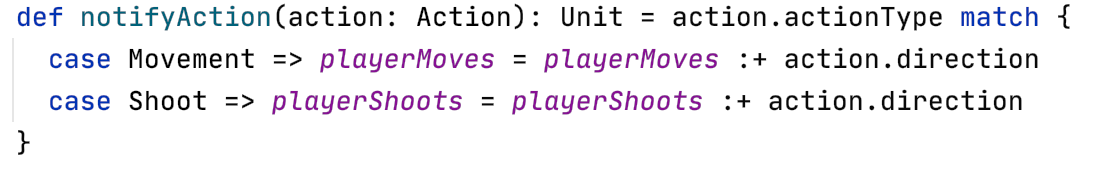
\includegraphics[width=13cm]{res/notifyAction.png}
      \caption{Aggiunge l'azione notificata alla relativa Queue}
      \label{notifyAction}
    \end{figure}
    
    \subsection{Testing Controller}
    Abbiamo creato i test riguardanti la parte del controller, utilizzando \textit{AnyFlatSpec} come tipologia di sintassi. 
    Abbiamo testato:
    
    \begin{itemize}
        \item La creazione della mappa di gioco all'avvio della partita.
        \item Il corretto riempimento delle queue di eventi relative al movimento e allo sparo.
        \item Il corretto dequeue degli eventi dalle due queue.
        \item La fine del gioco.
    \end{itemize}
    
    \subsection{Prolog}
    Abbiamo implementato il comportamento dei nemici utilizzando Prolog. Questa parte non è presente nella release finale in quanto, per mancanza di tempo, non è stata perfettamente integrata e comporta ancora qualche problema. Si trova, però, nel branch \textit{Prolog}.
    
    Sono stati creati due diversi tipi di nemici, distinti solamente dal loro \textit{movementBehaviour}, di seguito riportati:
    
    \subsubsection{EnemyWithRandomMove}
    Questa tipologia di nemico ha lo stesso behaviour implementato dai nemici presenti nella release attuale, come si evince dalla figura \ref{random}.
    
    \begin{figure}[H]
    \centering
      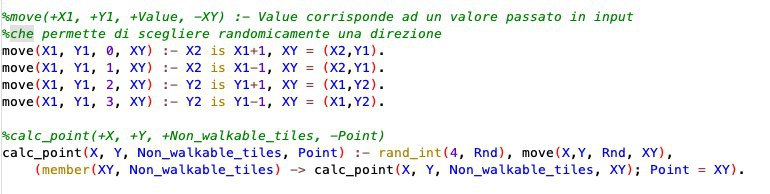
\includegraphics[width=15cm]{res/randomProlog.jpg}
      \caption{Random behaviour in Prolog}
      \label{random}
    \end{figure}
    
    \subsubsection{EnemyWithLeftRightMove}
    Questa tipologia di nemico si muove da destra verso sinistra e viceversa nelle caselle in cui può muoversi, invertendo il proprio senso di marcia quando incontra un ostacolo, come riportato in figura \ref{left}.
    
    \begin{figure}[H]
    \centering
      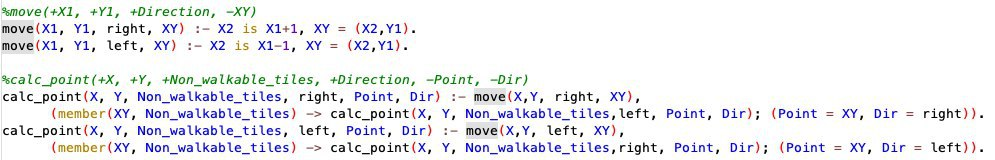
\includegraphics[width=16cm]{res/leftRightMove.jpg}
      \caption{LeftRight behaviour in Prolog}
      \label{left}
    \end{figure}
    
    \subsubsection{Problemi riscontrati}
    Con l'introduzione di Prolog, arrivati ad un certo numero di nemici, abbiamo riscontrato che l'applicazione mostra pesanti lag.
    Pensiamo che sia dovuto all'architettura dell'event-loop a single-thread. Per risolvere questo problema si dovrebbe rendere il clacolo delle nuove posizioni dei nemici, quindi lo svolgimento delle query Prolog, concorrente.